\chapter{Implementierung}
\label{cha:Implementierung}

In diesem Kapitel wird die Implementierung der systemtragenden Komponenten anhand von Codebeispielen erläutert. Dabei werden wichtige Gedanken und Überlegungen, die während des Entwicklungsprozesses entstanden sind, aufgegriffen und anhand der vorliegenden Implementierungen diskutiert. Ebenso wird das Ergebnis der Benutzeroberflächengestaltung und die dabei umgesetzten Konzepte beleuchtet.

\section{Server}

Die in Abschnitt \ref{sec:Entwurf:Server} vorgestellten Kernkomponenten der Serverarchitektur werden in diesem Abschnitt im Detail beleuchtet und dabei vor allem wichtige Implementierungen hinsichtlich der an die Webanwendung gestellten Anforderungen erläutert.

\subsection{Model}

In Abschnitt \ref{sec:Entwurf:Server} wurden Models bereits als Bestandteile der Datenzugriffsschicht eingeführt. Models sind dabei Klassen die Tabellen einer relationalen Datenbank hinsichtlich ihrer Eigenschaften, Schemata und Beziehungen beschreiben. Modelklassen erlauben es, zur Laufzeit der Anwendung objektorientierte Datenmodelle mit Hilfe eines Mappers in eine relationale Datenbank abzulegen. Die Funktion des Mappers übernimmt im Kontext dieser Implementierung das \acf{ORM} Framework Eloquent. Eloquent ist ein Bestandteil des Laravel PHP Frameworks, auf dem die gesamte serverseitige Implementierung aufbaut. Die Modelklassen werden gemäß den in Abschnitt \ref{sec:Analyse:Server} gestellten technologischen Anforderungen nach dem Database-First-Prinzip vollständig generiert. Als Generator wurde dabei die Bibliothek \emph{laravel-model-generator} verwendet, die die Funktionen des Eloquent Framework um die benötigte Funktionalität erweitert. Das Ergebnis einer solchen generierten Modelklasse wird in Listing \ref{prog:model} als Programmcode dargestellt.

\begin{program}[H]
% place caption consistently either at the top or bottom:
\begin{PhpCode}
<?php namespace App\Models;

use Illuminate\Database\Eloquent\Model;

class FilterFilterGroup extends Model {

    protected $primaryKey = 'filterGroupID';
    protected $table = 'Filter_FilterGroup';
    protected $fillable = ['shortName', 'displayName', 'infoTooltip', 'helpTooltip', 'initiallyCollapsed', 'displaySequence'];


    public function translation() {
        return $this->belongsTo(\App\Models\CommonTranslateWordId::class, 	'displayName', 'wordID');
    }

    public function filterFilters() {
        return $this->hasMany(\App\Models\FilterFilter::class,'filterGroupID','filterGroupID');
    }
}
\end{PhpCode}
\captionof{lstlisting}{Beispiel einer generierten Modelklasse}
\label{prog:model}
\end{program}

Im oberen Abschnitt der Klasse finden sich Merkmale und Eigenschaften, die das Schema der zugehörigen Datenbanktabelle beschreiben. Die dargestellten Funktionen beschreiben hingegen die Beziehung zu verknüpften Tabellen. Diese Beziehungen werden mithilfe von Funktionen modelliert, die vom Eloquent-Framework bereitgestellt werden. Jede Modelklasse leitet von einer Basismodelklasse ab. Diese Basismodelklasse implementiert wiederum ein Interface, mit dessen Hilfe die Datenbank angesprochen werden kann. Der Zugriff auf die Datenbank erfolgt dabei Model zentriert. Modelklassen bilden damit das Rückgrat der Serverimplementierung, indem sie es erlauben Daten aus Datenbankabfragen als Objekt zu kapseln, das im weiteren Verlauf im Kontext einer objektorientierten Implementierung genutzt werden kann.

\subsection{Controller}

Controller wurden in Abschnitt \ref{sec:Entwurf:Server} als Implementierung der Ressourcen des entwickelten RESTful Webservice. Controller implementieren Models um auf Grundlage der HTTP-Methoden, die auf einer Ressource aufgerufen werden können, konkrete Datenbankabfragen zu realisieren. Ein Controller beinhaltet bis auf wenige Ausnahmen immer genau vier Methoden: Lesen, Speichern, Löschen und Aktualisieren von Ressourcen. Um die Integration mit den Models zu erklären, wird in Listing \ref{prog:controller} als Beispiel eine eher komplexere Update-Methode dargestellt.

\begin{program}[H]
% place caption consistently either at the top or bottom:
\begin{PhpCode}
   public function update(FilterRequest $request, $id)
    {
        DB::beginTransaction();

        try {
            $input = $request->json()->all();
            $filter = Filter::with('translation.en')->findOrFail($id);
            $group = FilterGroup::findOrFail($input['group']['id']);
            $type = FilterType::findOrFail($input['type']['id']);
            $productGroup = ProductGroup::findOrFail($input['productGroup']['id']);

            $filter->translation->en->first()->word = $input['name'];
            $filter->shortName = $input['shortName'];
            $filter->filterDisplaySequence = $input['sequence'];

            $filter->group()->associate($group);
            $filter->type()->associate($type);
            $filter->productGroup()->associate($productGroup);

            if ($filter->push()) {
                DB::commit();
                return $this->item($filter, new FilterTransformer());
            }
        } catch (\Exception $e) {
            DB::rollback();
            throw $e;
        }
    }
\end{PhpCode}
\captionof{lstlisting}{Beispiel einer Update-Methode aus einem API-Controller}
\label{prog:controller}
\end{program}

Die dargestellte Methode realisiert die Aktualisierung einer Filter-Ressource. Das über die Schnittstelle gesendete, zu aktualisierende Filterobjekt, wird als Request-Objekt gekapselt und neben der ID an die Update-Methode übergeben. Die Update-Methode implementiert die entsprechenden Modelklassen um den Aktualisierungsvorgang zu realisieren. Eine Besonderheit dabei ist, dass Operationen, die Daten in die Datenbank schreiben, immer in einem Transaktionsblock definiert sind. Das hat den Vorteil, dass es quasi ausgeschlossen ist, aufgrund von fehlerhaften Abfragen einen inkonsistenten Datenbankzustand zu provozieren. Wenn auf Datenbankebene ein Fehler auftritt, wird die laufende Transaktion abgebrochen und der ursprüngliche Zustand der Datenbank wiederhergestellt.

In Programmzeile 6 bis 10 wird anhand von Modelklassen das zu aktualisierende Filterobjekt und ebenfalls die zu aktualisierenden Relationen geladen. Konnten die Relationen gefunden bzw. geladen werden, werden diese mit dem Filterobjekt verknüpft (Programmzeile 16-18) und anschließend das aktualisierte Filterobjekte persistiert (Programmzeile 20). Eine Besonderheit ergibt sich aus der in Programmzeile 22 definierten Rückgabefunktion, die einen sogenannten Transformer aufruft und damit die Überleitung zu den in Abschnitt \ref{sec:imp:Transformer} betrachteten Transformern herstellt.

\subsection{Transformer}
\label{sec:imp:Transformer}

Transformer wurden in Abschnitt \ref{sec:Entwurf:Server} als Komponenten zur Homogenisierung und Standardisierung von Rohdaten eingeführt. Die im vorherigen Abschnitt beschriebenen Controller-Methoden definieren alle einen Rückgabewert. Diese Rückgabewerte sind immer Repräsentationen von Ressourcen im Kontext der jeweiligen aufgerufenen Methode und werden immer durch einen Transformer realisiert. Das bedeutet, das Transformer die Repräsentation einer Ressource hinsichtlich des Inhalts und Formats bestimmen. Eine Transformer-Klasse wird in der Regel immer von genau einem Controller implementiert. Sie haben die Aufgabe, die aus den Abfragen der Modelklassen resultierenden Rohdaten in ein für den RESTful Webservice geeignet Format zu überführen. Dieser Vorgang wird in Listing
\ref{prog:transformer} exemplarisch dargestellt. Um logisch an das gegebene Beispiel aus Abbildung \ref{prog:controller} anzuschließen wurde ein Ausschnitt aus der korrespondierende FilterTransformer-Klasse gewählt. 

\begin{program}[H]
% place caption consistently either at the top or bottom:
\begin{PhpCode}
public function transform(Filter $filter)
    {
        return [
            'id' => (int) $filter->filterID,
            'name' => $filter->translation->en->first()->word,
            'shortName' => $filter->shortName,
            'sequence' => (int) $filter->filterDisplaySequence,
            'spaceLeft' => (int) $filter->filterSpaceLeftInPixel,
            'spaceRight' => (int) $filter->filterSpaceRightInPixel
        ];
    }
\end{PhpCode}
\captionof{lstlisting}{Beispiel einer Transform-Methode aus einer Transformer-Klasse}
\label{prog:transformer}
\end{program}

Die Methode \emph{transform()} wird in diesem Beispiel mit einem Modelobjekt vom Typ Filter aufgerufen. Anhand von Zugriffen, die über die Modelklasse realisiert werden, kann so ein Rückgabeobjekt mit beliebigen Inhalt und Format modelliert werden. Dabei geht es aber nicht nur um simple Anpassung von Bezeichnern, wie zum Beispiel in Programmzeile 4 geschehen\footnote{An dieser Stelle wird, die aus der Datenbank kommende \emph{filterID}, auf das Feld \emph{id} gemappt. Das Mapping von ID's geschieht in jedem Transformator nach demselben Schema und beschreibt einen Teil der Datenhomogenisierung.}, sondern auch um Mapping-Funktionen\footnote{Als Mapping wird der Prozess bezeichnet, der Datenelemente zwischen unterschiedlichen Datenmodellen abbildet.} über Relationen hinweg. In Programmzeile 5 erfolgt ein solches relationales Mapping, indem die englische Übersetzung des Anzeigenamens des übergebenden Filterobjekts aus der Translation-Tabelle geladen und auf das Feld \emph{name} gemappt wird. Zusammenfassend lassen sich also zwei Kernaufgaben der Transformatoren herausstellen:

\begin{itemize}
\item Die Konvertierung von Rohdaten, in ein für die Schnittstelle geeignetes Format
\item Die Realisierung von benötigten Abhängigkeiten über das nachladen von in Beziehung stehenden Datenobjekten oder -feldern.
\end{itemize}

\subsection{Router}

Der Router wurde in Abschnitt \ref{sec:Entwurf:Server} als die Komponente beschrieben, die die Schnittstelle des entwickelten Webservice realisiert. Der Router realisiert die Schnittstellenspezifikation, in dem er alle verfügbaren Endpunkte und die jeweils aufrufbaren HTTP-Methoden implementiert. Wird ein Endpunkt von einem Client aufgerufen, werden die ankommenden Daten automatisch durch das Laravel Framework in ein Request-Objekt geschrieben. Dieses Request-Objekt enthält neben allen Informationen, die im HTTP-Header und Body übertragen werden, auch Metainformationen über das verwendete Datenformat. Außerdem stellt ein Request-Objekt unter anderem auch Helferfunktionen zur Verfügung, um die Daten aus dem HTTP Message Body zu parsen. Die Schnittstelle implementiert als Datenformat \acf{JSON}, ist aber so flexibel gestaltet, dass serverseitig auch eine problemlose Umstellung auf \ac{XML} erfolgen kann. Der Einsatz von \ac{JSON} als Datenformat macht im Kontext eines auf Javascript basierenden Webfrontend aber in jedem Fall Sinn, da clientseitig JSON-Objekte ohne weiteres Zutun in Javascript-Objekte umgewandelt werden können. 

Der Router implementiert außerdem sogenannte Middlewares, die bestimmte Funktionen auf einer festgelegten Gruppe von Endpunkten ausführen. Über eine Authentifizierungsmiddleware erfolgt beispielsweise die Absicherung der Schnittstelle. Das in Abbildung \ref{fig:authentification} dargestellte Sequenzdiagramm beschreibt Auszugsweise den Vorgang der Authentifizierung.
\begin{figure}[H]
\centering
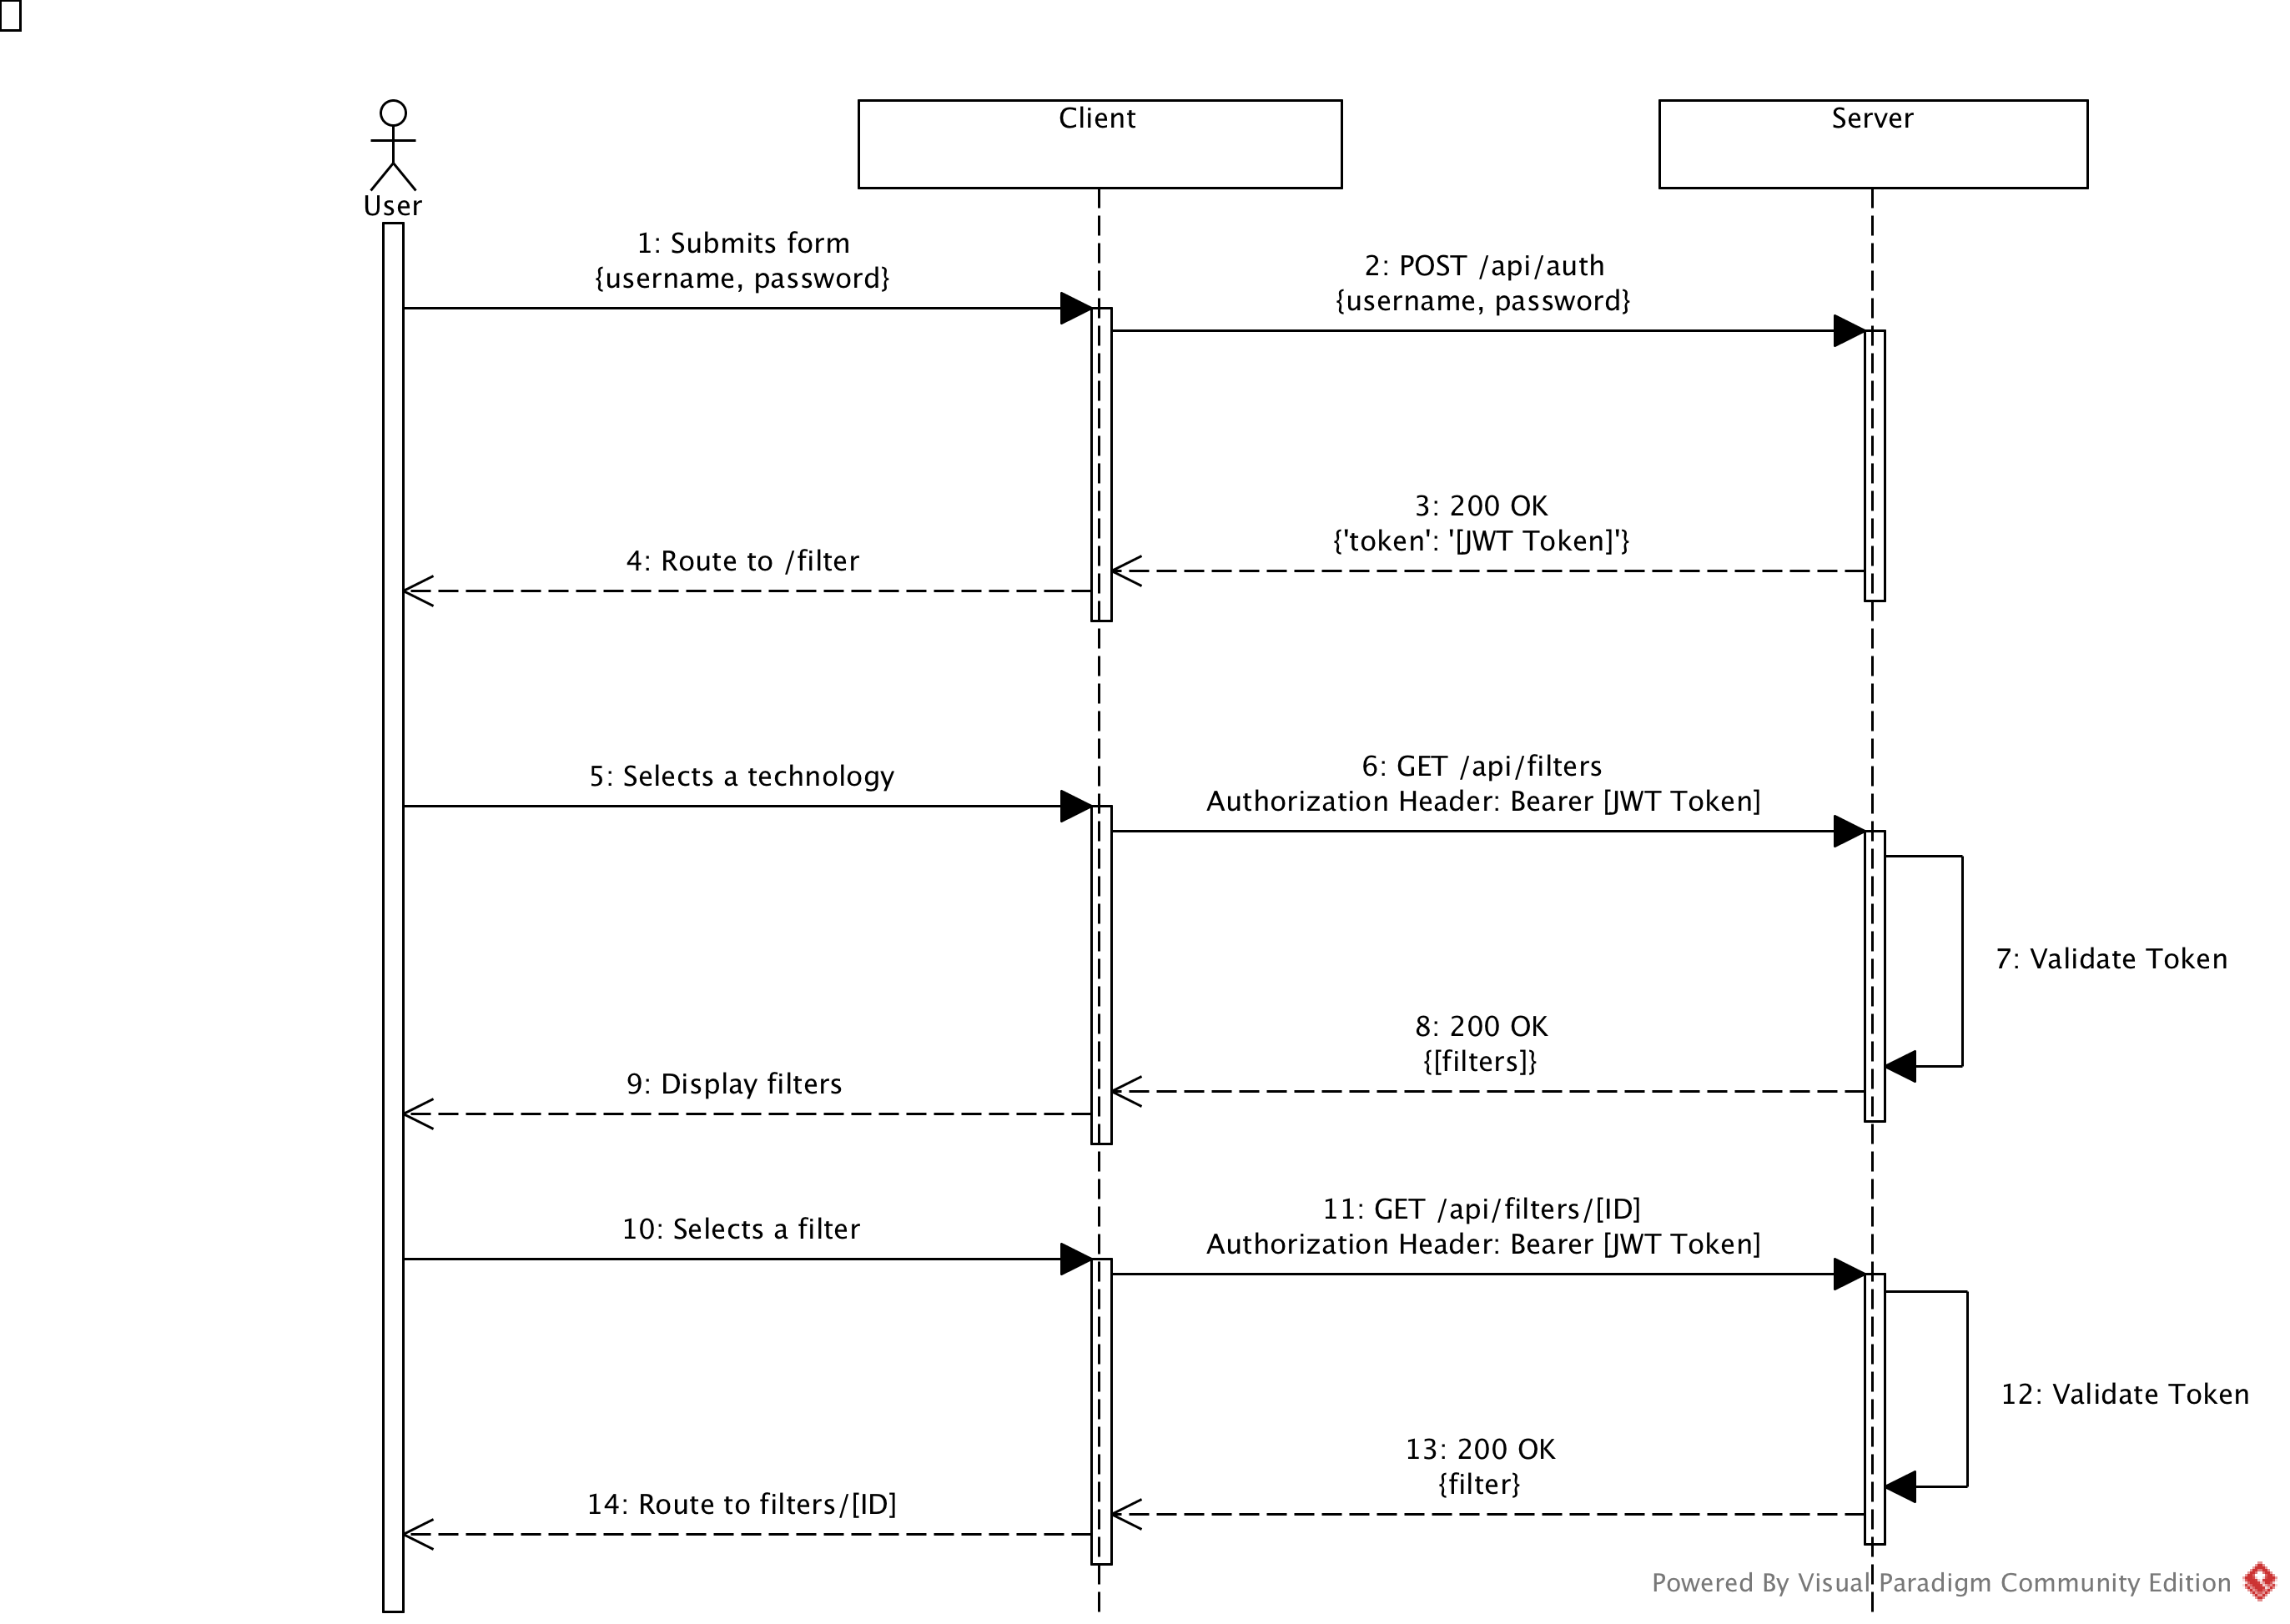
\includegraphics[width=1.0\textwidth]{authentification} %{CS0031}
\caption{Tokenbasierte Authentifizierung}
\label{fig:authentification}
\end{figure}
Die Authentifizierung am Server erfolgt über die in Abschnitt \ref{sec:ROA:Sicherheit} vorgestellten tokenbasierten Authentifizierung. Ein Benutzer muss sich nach der in Abschnitt \ref{sec:Funktionale Anforderungen} gestellten Anforderung \glqq{}\emph{Anmelden}\grqq{} an der Webanwendung anmelden, um deren Funktionalität nutzen zu können. Die Anmeldung erfolgt über einen Benutzernamen und ein Passwort. Die eingegebenen Anmeldedaten werden serverseitig mit einer User-Tabelle abgeglichen. Sind die Anmeldedaten korrekt, wird von der Authentifizierungsmiddleware ein Token generiert, der mit einem geheimen Schlüssel signiert wird. Dieser Token wird als Antwort zurück an den Client geschickt, der das Token in einem sogenannten Cookie ablegt. Durch die Ablage des Tokens in einem Browser-Cookie, kann der Benutzer zwischenzeitlich auch seinen Browser schließen und bei erneutem Besuch der Webanwendung den selben Token wiederverwenden; der Benutzer muss sich also nicht noch einmal neu Anmelden, solange der Token noch gültig ist. In dem dargestellten Sequenzdiagramm werden beispielhaft weitere Interaktionen des Benutzer und Aufrufe des Clients dargestellt. Dadurch soll ausgedrückt werden, dass der Token ab der Anmeldung in jedem HTTP-Request als Teil des Header mitgesendet wird. Auch die Validierung des Tokens erfolgt bei jedem Aufruf einer geschützten Ressource. Anhand dieser Implementierung wird eine sichere und zustandslose Art der Authentifizierung realisiert.

\section{Client}

Die Frontend-Komponente der Webanwendung wurde mit dem Javascript-Framework \mbox{AngularJS} entwickelt. In Abschnitt \ref{sec:Entwurf:Client} wurde bereits ausgeführt, dass \mbox{AngularJS} ein klassisches MVC-Architekturmuster als \ac{SPA} realisiert. Schwerpunkt der nachfolgenden Abschnitte bildet die Betrachtung der einzelnen Frontend-Komponenten und ihrer Rollen im Kontext der Gesamtanwendung. Außerdem wird das Ergebnis der Benutzeroberflächenimplementierung anhand ausgewählter Aspekte beleuchtet.

\subsection{Model}

Das Model enthält die darzustellenden Daten und ist von Präsentation und Steuerung unabhängig. Models werden im Kontext von AngularJS typischerweise an einer Variable \emph{\$scope} definiert. Dies kann sowohl innerhalb eines Controllers als auch direkt im View über eine sogenannte Direktive erfolgen. Direktiven realisieren Funktionen, die das Vokabular von HTML erweitern. Mittels Direktiven können neue HTML-Tags und Attribute erstellt oder durch bestimmte Funktionalität erweitert werden. Über ein sogenanntes Two-Way-Databinding, das von AngularJS realisiert wird, können Models sowohl im Controller als auch im View verändert werden. Die jeweils andere Komponente wird dann über die Änderung benachrichtigt und kann sich aktualisieren. Die Implementierung von Models beschränkt sich im Falle der Webanwendung auf einfache Variablen die am \emph{\$scope} gespeichert werden. Das sind vor allem Daten, die über den Webservice geladen und in Form von Javascript-Objekten nutzbar gemacht werden. Die Definition solcher \emph{\$scope} Variablen erfolgt im Falle der Webanwendung fast ausschließlich in den jeweiligen Controllern, um eine bessere Übersicht zu gewährleisten. Die Models der Webanwendung realisieren dabei im wesentlichen folgende Funktionen:

\begin{itemize}
\item Generierung der datengetriebenen Filtersteuerelemente, indem die Modeldaten an entsprechende Direktiven übergeben werden. Diese Direktiven realisieren dann die konkrete Ausprägung des Filtersteuerelements (Dropdown-Liste oder Schalter)
\item Schnittstelle zwischen Dateneingabemasken (Formularen) und Controller-Logik, indem Models über Direktiven an Formularelemente gebunden werden.
\end{itemize}

\subsection{Repository}
\label{sec:imp:Respository}

Das Repository bildet das Gegenstück, der auf der serverseite realisierten Router-Komponente. Das Repository kapselt alle Endpunkte der Schnittstelle, die das Webfrontend für die Erfüllung seiner Aufgaben benötigt. Der Zugriff auf die Schnittstelle wurde mit Hilfe der Javascript-Bibliothek \emph{Restangular} realisiert. Restangular simplifiziert den Zugriff auf eine REST-konforme Schnittstelle wesentlich. So ist es zum Beispiel möglich eine Ressource Filter mit minimalen Aufwand durch den folgenden Aufruf anzusteuern.
\begin{JsCode}[numbers=none]
     getFilter: function(id, params) {
                    return Restangular.one('filters', id).get(params);
                },
\end{JsCode}
In diesem Beispiel wird aus dem in der Methode \emph{one()} übergebenen URI-Bestandteilen der Zugriff auf die Schnittstelle vollautomatisch durch Restangular realisiert. Das zurückgegebene Objekt beinhaltet neben den erwarteten Filterdaten auch Methoden zum Manipulieren des Objekts. So kann das Filterobjekt zum Beispiel im Verlauf der Anwendung modifiziert werden und anschließend einfach eine Methode \emph{save()} direkt auf dem Objekt aufgerufen werden. Anhand der an dem Objekt gespeicherten Metadaten, kann Restangular den Zugriff auf die Ressource zum Speichern der Daten ableiten und vollautomatisch realisieren. Ein manuelles Implementieren von Funktionen zum Speichern, Löschen oder Aktualisieren von Ressourcen entfällt damit clientseitig vollständig. 

\subsection{Controller}

Im Gegensatz zu den serverseitigen Controllern, haben die Controller auf der Clientseite keinen klar abgegrenzten Aufgabenbereich. Geht man nach den Empfehlungen von AngularJS sollten Controller lediglich die Bindung von Datenobjekten an die \emph{\$scope} Variable realisieren. Die Controller implementieren diesen Sachverhalt, indem sie über ein Repository mittels eines \ac{AJAX}-Aufrufs den Webservice ansprechen und das Ergebnis an den besagten \emph{\$scope} binden. Außerdem implementieren Controller auch die Geschäftslogik der Clientseite, die zum Beispiel für die Modifizierung von Datenstrukturen oder anderen aufgabenrelevanten Sachverhalten benötigt wird. Einer dieser Sachverhalte im Kontext der in Abschnitt \ref{sec:Funktionale Anforderungen} ermittelten funktionalen Anforderungen ist von besonderer Wichtigkeit und wird daher nachfolgend im Detail betrachtet. Die funktionale Anforderung \glqq{}\emph{Filter anzeigen}\grqq{} aus Abschnitt \ref{sec:Funktionale Anforderungen} lautet: 
\begin{quote}
Filtersteuerelemente müssen dem Benutzer angezeigt werden. Die Anwendung generiert die Filtersteuerelemente anhand der Filterdaten und orientiert sich dabei am Layout des FlowConfigurator. Die Anzeige muss zusätzlich Schaltflächen, für die auf die Filter anwendbaren Operationen enthalten (Bearbeiten, Löschen, Erstellen).
\end{quote}
Diese Anforderung impliziert eine besondere Herausforderung an die datengestützte Generierung der Filtersteuerelemente im Webfrontend. Die in der Datenbasis vorliegenden layoutspezifischen Daten, die die Anordnung der Filtersteuerelemente beschreiben, basieren auf einem Fließlayout. Das bedeutet, dass in der FlowConfigurator Software Filtersteuerelemente einfach nacheinander in einen dafür vorgesehenen Container geladen werden (siehe Abbildung \ref{fig:layout}) und dabei benötigte Abstände zwischen Filtersteuerelementen über Pixelangaben realisiert werden. Diese Pixelangaben sind Teil der layoutspezifischen Daten und werden direkt in der Filtertabelle gespeichert. Aufgrund der in Abschnitt \ref{sec:Analyse:Nichtfuntionale Anforderungen} aufgestellten Anforderung an die Portabilität, die unter anderem besagt, dass die Webanwendung möglichst auch auf kleinen Bildschirmen korrekt dargestellt werden soll, wurde sich für die Darstellung der Filtersteuerelemente in einem Grid-Layout entschieden. Dieses Grid-System wurde mit Hilfe des Frontend Frameworks Bootstrap realisiert und bietet den Vorteil das Spalten und Zeilen definiert werden können, die je nach Bildschirmgröße korrekt umbrechen und damit eine solide Basis eines responsiven Layouts bilden. Die Herausforderung liegt nun darin begründet, aus den Daten eines Fließlayouts, ein Grid-Layout zu generieren, dass die Filtersteuerelemente exakt so anzeigt werden, wie in der FlowConfigurator Software. Zu diesem Zweck wurden die Filterdaten eingehend analysiert und anhand von Oberflächentests ermittelt, nach welchem Muster die Filtersteuerelemente im FlowConfigurator angezeigt werden. Dabei konnte festgestellt werden, dass die FlowConfigurator Software stehts ein zwei- oder dreispaltiges Layout simuliert. Anhand dieser Erkenntnis wurden Regeln formuliert, die die Grundlage generischer Algorithmen bilden, welche anhand der gegebenen Filterdaten im Webfrontend ermitteln können, ob die Filtersteuerelemente in einem zwei- oder dreispaltigen Layout angezeigt werden sollen. Zusammenfassend lässt sich der Prozess der datengetriebenen Generierung der Filterelemente damit durch folgende Punkte:

\begin{enumerate}
\item Filterdaten werden über die Schnittstelle geladen
\item Ein Algorithmus bestimmt ob ein zwei- oder dreispaltiges Layout für die Darstellung der Filtersteuerelemente verwendet werden soll
\item Die Filtersteuerelemente werden auf Basis des ermittelten Layouts generiert und Abstände zwischen Elementen die größer als eine Spalte sind durch Platzhalterelemente ersetzt
\end{enumerate}
Das Ergebnis dieser Implementierung wird im Abschnitt \ref{sec:imp:Benutzeroberfläche} dargestellt.

\subsection{Router}

Der Router ist die Kernkomponente des Clients und definiert alle \ac{URL}'s die innerhalb des Client-Frontend aufgerufen werden können. In Abschnitt \ref{sec:Entwurf:Client} wurde bereits erörtert, dass sich der Router aus sogenannten States zusammensetzt, welche das Zusammenspiel der einzelnen Client-Komponenten orchestrieren. Anhand des in Listing dargestellten Programmcodes wird der Aufbau eines solchen States beispielhaft erläutert.
\begin{program}[H]
% place caption consistently either at the top or bottom:
\begin{JsCode}
$stateProvider
.state('app.filters.edit', {
    url: '/filters/{fId:int}',
    ncyBreadcrumb: {
        label: function ($stateParams) {
            return $stateParams.fId
        }
    },
    views: {
        'content@app': {
            templateUrl: 'app/app/filter/edit/edit.html',
            controller: 'FilterEditCtrl'
        }
    },
    resolve: {
        filter: function (Repository, $stateParams) {
            return Repository.getFilter($stateParams.fId).then(function (res) {
                return res.data.plain();
            })
        },
        types: function (Repository) {
            return Repository.getFilterTypes().then(function (res) {
                return res.data.plain();
            })
        },
        groups: function (Repository) {
            return Repository.getFilterGroups().then(function (res) {
                return res.data.plain();
            })
        },
        productGroups: function (Repository) {
            return Repository.getProductGroups().then(function (res) {
                return res.data.plain();
            })
        },
    }
})
\end{JsCode}
\captionof{lstlisting}{Beispiel eines Router-States}
\label{prog:router}
\end{program}
Ein State ist ein Mittel zur Beschreibung von Vorgängen, die beim Aufruf einer bestimmten Route erfolgen. Der dargestellte State besteht aus vier Bestandteilen, die nachfolgend getrennt voneinander betrachtet werden.

\subsubsection{URL}

Die Funktion \emph{url} bestimmt die \ac{URL}, die aufgerufen werden muss um den State zu \glqq{}aktivieren\grqq{}. Dieser Parameter kann auch dynamische Bestandteile enthalten. Zum Beispiel wird in Programmzeile 3 ein Parameter als Bestandteil der \ac{URL} definiert. Diese Parameter lassen sich ebenfalls typisieren. Im vorliegenden Beispiel wird der State nur aktiviert, wenn der Parameter ein Integer-Wert ist. Die Parameter werden durch ui-router ausgelesen und können im weiteren Verlauf der Anwendung für verschiedene Zwecke genutzt werden.

\subsubsection{Views}

Die Funktion \emph{views} gibt an, welche HTML-Templates beim Aufruf eines States geladen und wo auf der Webseite sie angezeigt werden sollen. Ein Template kann dabei mit einem Controller verknüpft werden. Für rein statische Templates kann die Verknüpfung mit einem Controller aber auch entfallen. Bezogen auf den Beispielcode wird ein Template zur Bearbeitung von Filterdaten geladen, das mit einem korrespondierenden Controller verknüpft wird.

\subsubsection{Resolve}

Der Parameter resolve ist ein Mittel um Abhängigkeiten vor dem Darstellen eines HTML-Templates und vor dem Aufruf eines möglichen verknüpften Controllers aufzulösen. Im Falle des Beispiels wird die Resolve-Funktion in Programmzeile 15-36 für das Laden von Daten über den Webservice benutzt. Zu diesem Zweck wird das Respository implementiert. Eine Besonderheit stellt der Aufruf in Programmzeile 17 dar. Hier wird aufbauend auf dem Beispiel aus Abschnitt \ref{sec:imp:Respository} ein Filter mit einer bestimmten ID geladen. Die ID ist dabei der dynamische Bestandteil aus der vorher definierten \ac{URL}. Dieses Konzept wird in vielen States der Webanwendung angewandt und erlaubt es damit sogar indirekt das Verhalten der Webanwendung in Bezug auf die Schnittstelle des Webservice zu steuern. Beispielsweise könnte ein Benutzer, wenn er die ID eines bestimmten Filterobjektes wüsste, diese direkt an die \ac{URL} anhängen und auf die entsprechende Seite für die Bearbeitung genau dieses Filters gelangen.

\subsubsection{ncyBreadcrumb}

Die Funktion ncyBreadcrumb ist eine eigene Erweiterung der State-Funktionalität, um eine sogenannte Breadcrumb-Navigation zu realisieren. Eine Breadcrumb-Navigation stellt die Navigationshierarchie dar, mit Hilfe derer ein Benutzer erfährt, wo genau er sich innerhalb der Webanwendung befindet. Diese Implementierung ist ein direkter Lösungsansatz um die in Abschnitt \ref{sec:Analyse:Identifizierung von Layout-Komponenten} identifizierte benötigte Layout-Komponente Nummer 2 zu realisieren.

\subsection{Benutzeroberfläche}
\label{sec:imp:Benutzeroberfläche}

Die Benutzeroberfläche setzt sich aus einzelnen Views (HTML-Templates) zusammen, deren Komposition über die Router-Komponente gesteuert wird. Für die Realisierung der Benutzeroberfläche wurde das Frontend Framework Bootstrap eingesetzt. Die in Abschnitt \ref{sec:Funktionale Anforderungen} gestellten funktionalen Anforderungen dienen maßgeblich als Orientierung für die benötigten und zu gestaltenden HTML-Templates. Das Ergebnis dieses Prozesses wird als Screenshot der Benutzeroberfläche in Abbildung \ref{fig:userinterface} dargestellt.
\begin{figure}[H]
\centering
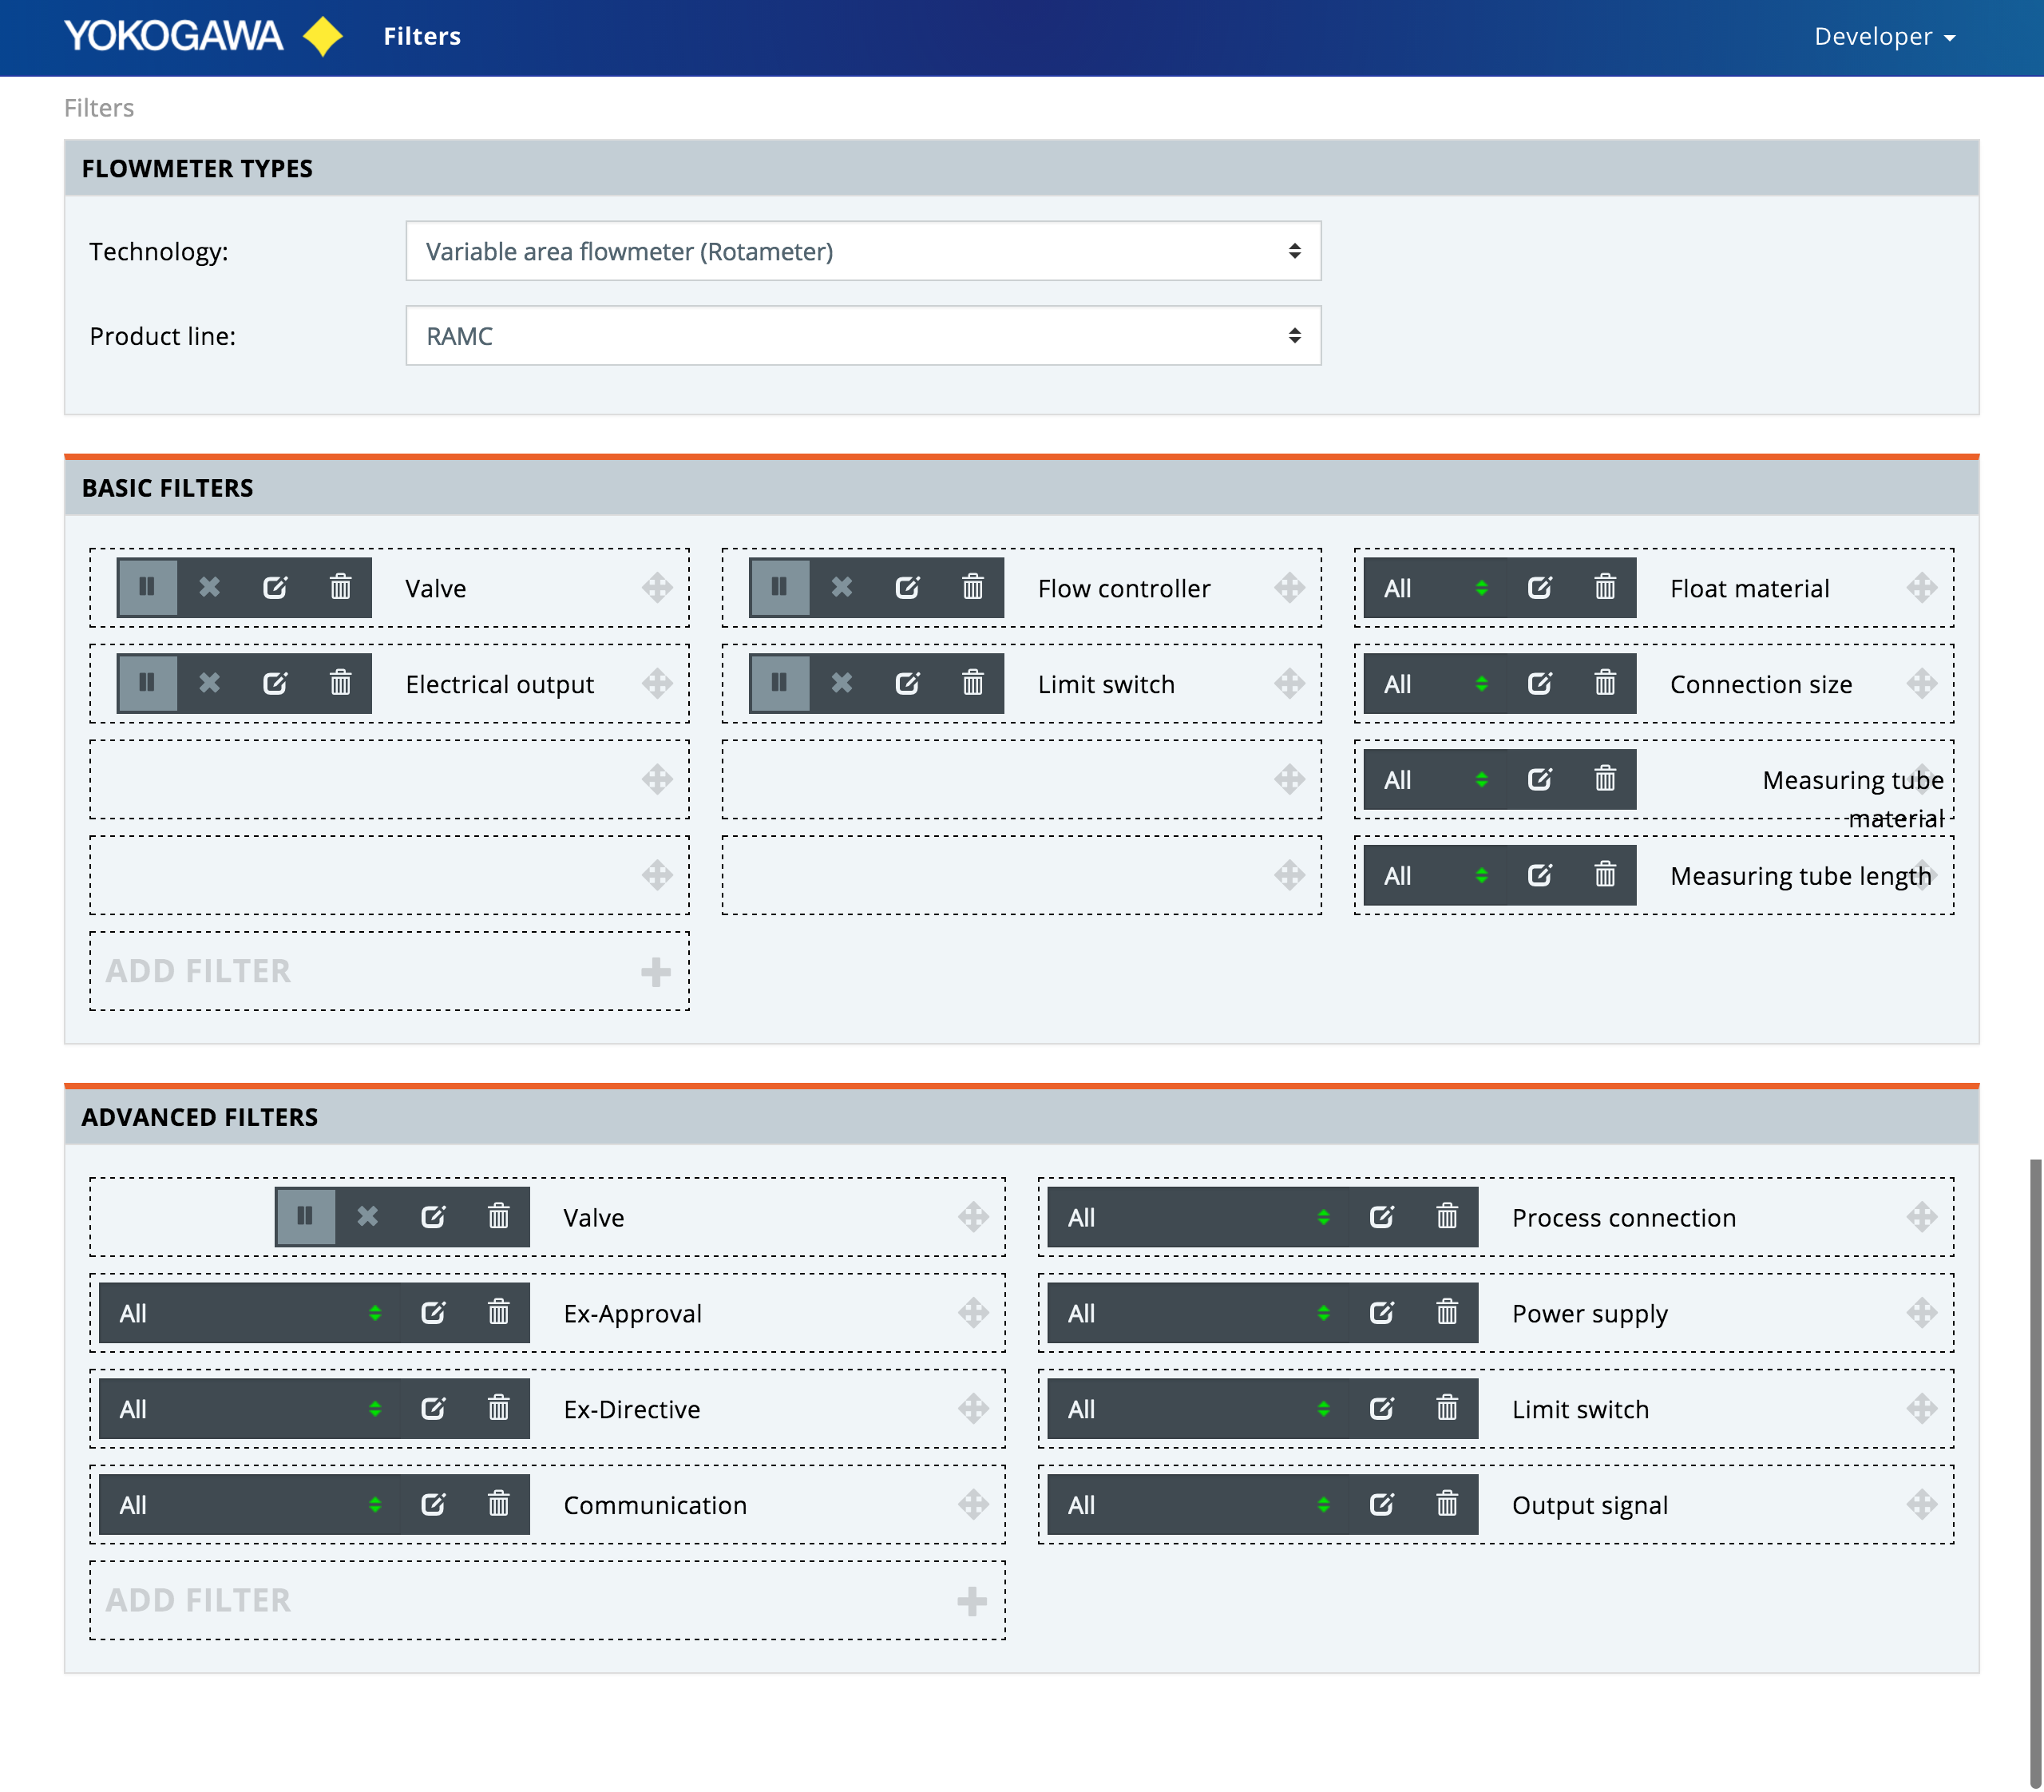
\includegraphics[width=1.0\textwidth]{ydm-index} %{CS0031}
\caption{Screenshot der Filterübersicht der Webanwendung.}
\label{fig:userinterface}
\end{figure}
Nachfolgend werden die realisierten View-Komponenten, aus denen sich die Benutzeroberfläche zusammensetzt, mit den gestellten Anforderungen abgeglichen und wichtige Konzepte und Gedanken zur Gestaltung diskutiert. Hauptanforderung an die Benutzeroberfläche war die inhaltliche und gestalterische Nähe zur FlowConfigurator Software. Dabei ging es keinesfalls darum eine exakte Kopie der Benutzeroberfläche der FlowConfigurator Software zu entwickeln, sondern durch den bedachten Einsatz von übergreifenden Gestaltungsmerkmalen und stilistischen Mitteln einen ähnlichen \glqq{}Look and Feel\grqq{} zu erzeugen. Die in Abschnitt \ref{sec:Analyse:Identifizierung von Layout-Komponenten} identifizieren und zu übernehmende Layout-Komponenten wurden umgesetzt und an die Anforderungen einer modernen Webanwendung angepasst. Das Hauptaugenmerk lag dabei auf der Gestaltung der Layoutkomponenten für die Anzeige der Filtersteuerelemente. Wie auf dem Screenshot in Abbildung \ref{fig:userinterface} zu erkennen ist, wurden die Filtersteuerelemente im Vergleich zur FlowConfigurator Software vergrößert, um eine bessere Bearbeitbarkeit zu gewährleisten. Die Steuerelemente wurden außerdem durch Buttons erweitert, die es erlauben Funktionen, auf Grundlage der in Abschnitt \ref{sec:Funktionale Anforderungen} ermittelten Kernanforderungen, direkt auf dem jeweiligen Steuerelement auszuführen. Das Aussehen der Steuerelemente wurde mittels \ac{CSS} an das Erscheinungsbild im FlowConfigurator angeglichen. Nur durch den Einsatz von \ac{CSS} konnten sogar normale HTML-Checkboxen als Schalter nach der Vorlage im FlowConfigurator realisiert werden.

Die Filtersteuerelemente werden vollständig datengetrieben in einem Grid-Layout generiert. Dieses Grid-Layout realisiert außerdem, einen Drag-and-Drop Funktionalität zum Verschieben der Filtersteuerelemente auf Basis der in Abschnitt \ref{sec:Entwurf:WYSIWYG als Gestaltungskonzept} erfolgten Vorbetrachtung. Die Drag-and-Drop Funktionalität wird in der Benutzeroberfläche durch die Umrandung der Filtersteuerelemente und einem entsprechenden Icon gekennzeichnet. Der Benutzer kann die Steuerelemente frei in dem dafür vorgesehenen Grid-Layout, das durch Platzhalterelemente ergänzt wird, verschieben. Das Verschieben der Steuerelemente funktioniert zudem auch über Filtergruppen hinweg. So ist es zum Beispiel möglich, einen Basisfilter in den Container der erweiterten Filter zu verschieben. Die entsprechenden Datenanpassungen werden im Hintergrund vorgenommen und müssen anschließend vom Benutzer über einen Dialog bestätigt werden.  

Neben der auf WYSIWYG basierenden Implementierung der Bearbeitung von Filtersteuerelement mit Hilfe direkter Manipulation, wurden außerdem HTML-Templates für die Bearbeitung der Geschäftsdaten entworfen. In Abbildung \ref{fig:editpage} wird solch eine Seite als Screenshot dargestellt.
\begin{figure}[H]
\centering
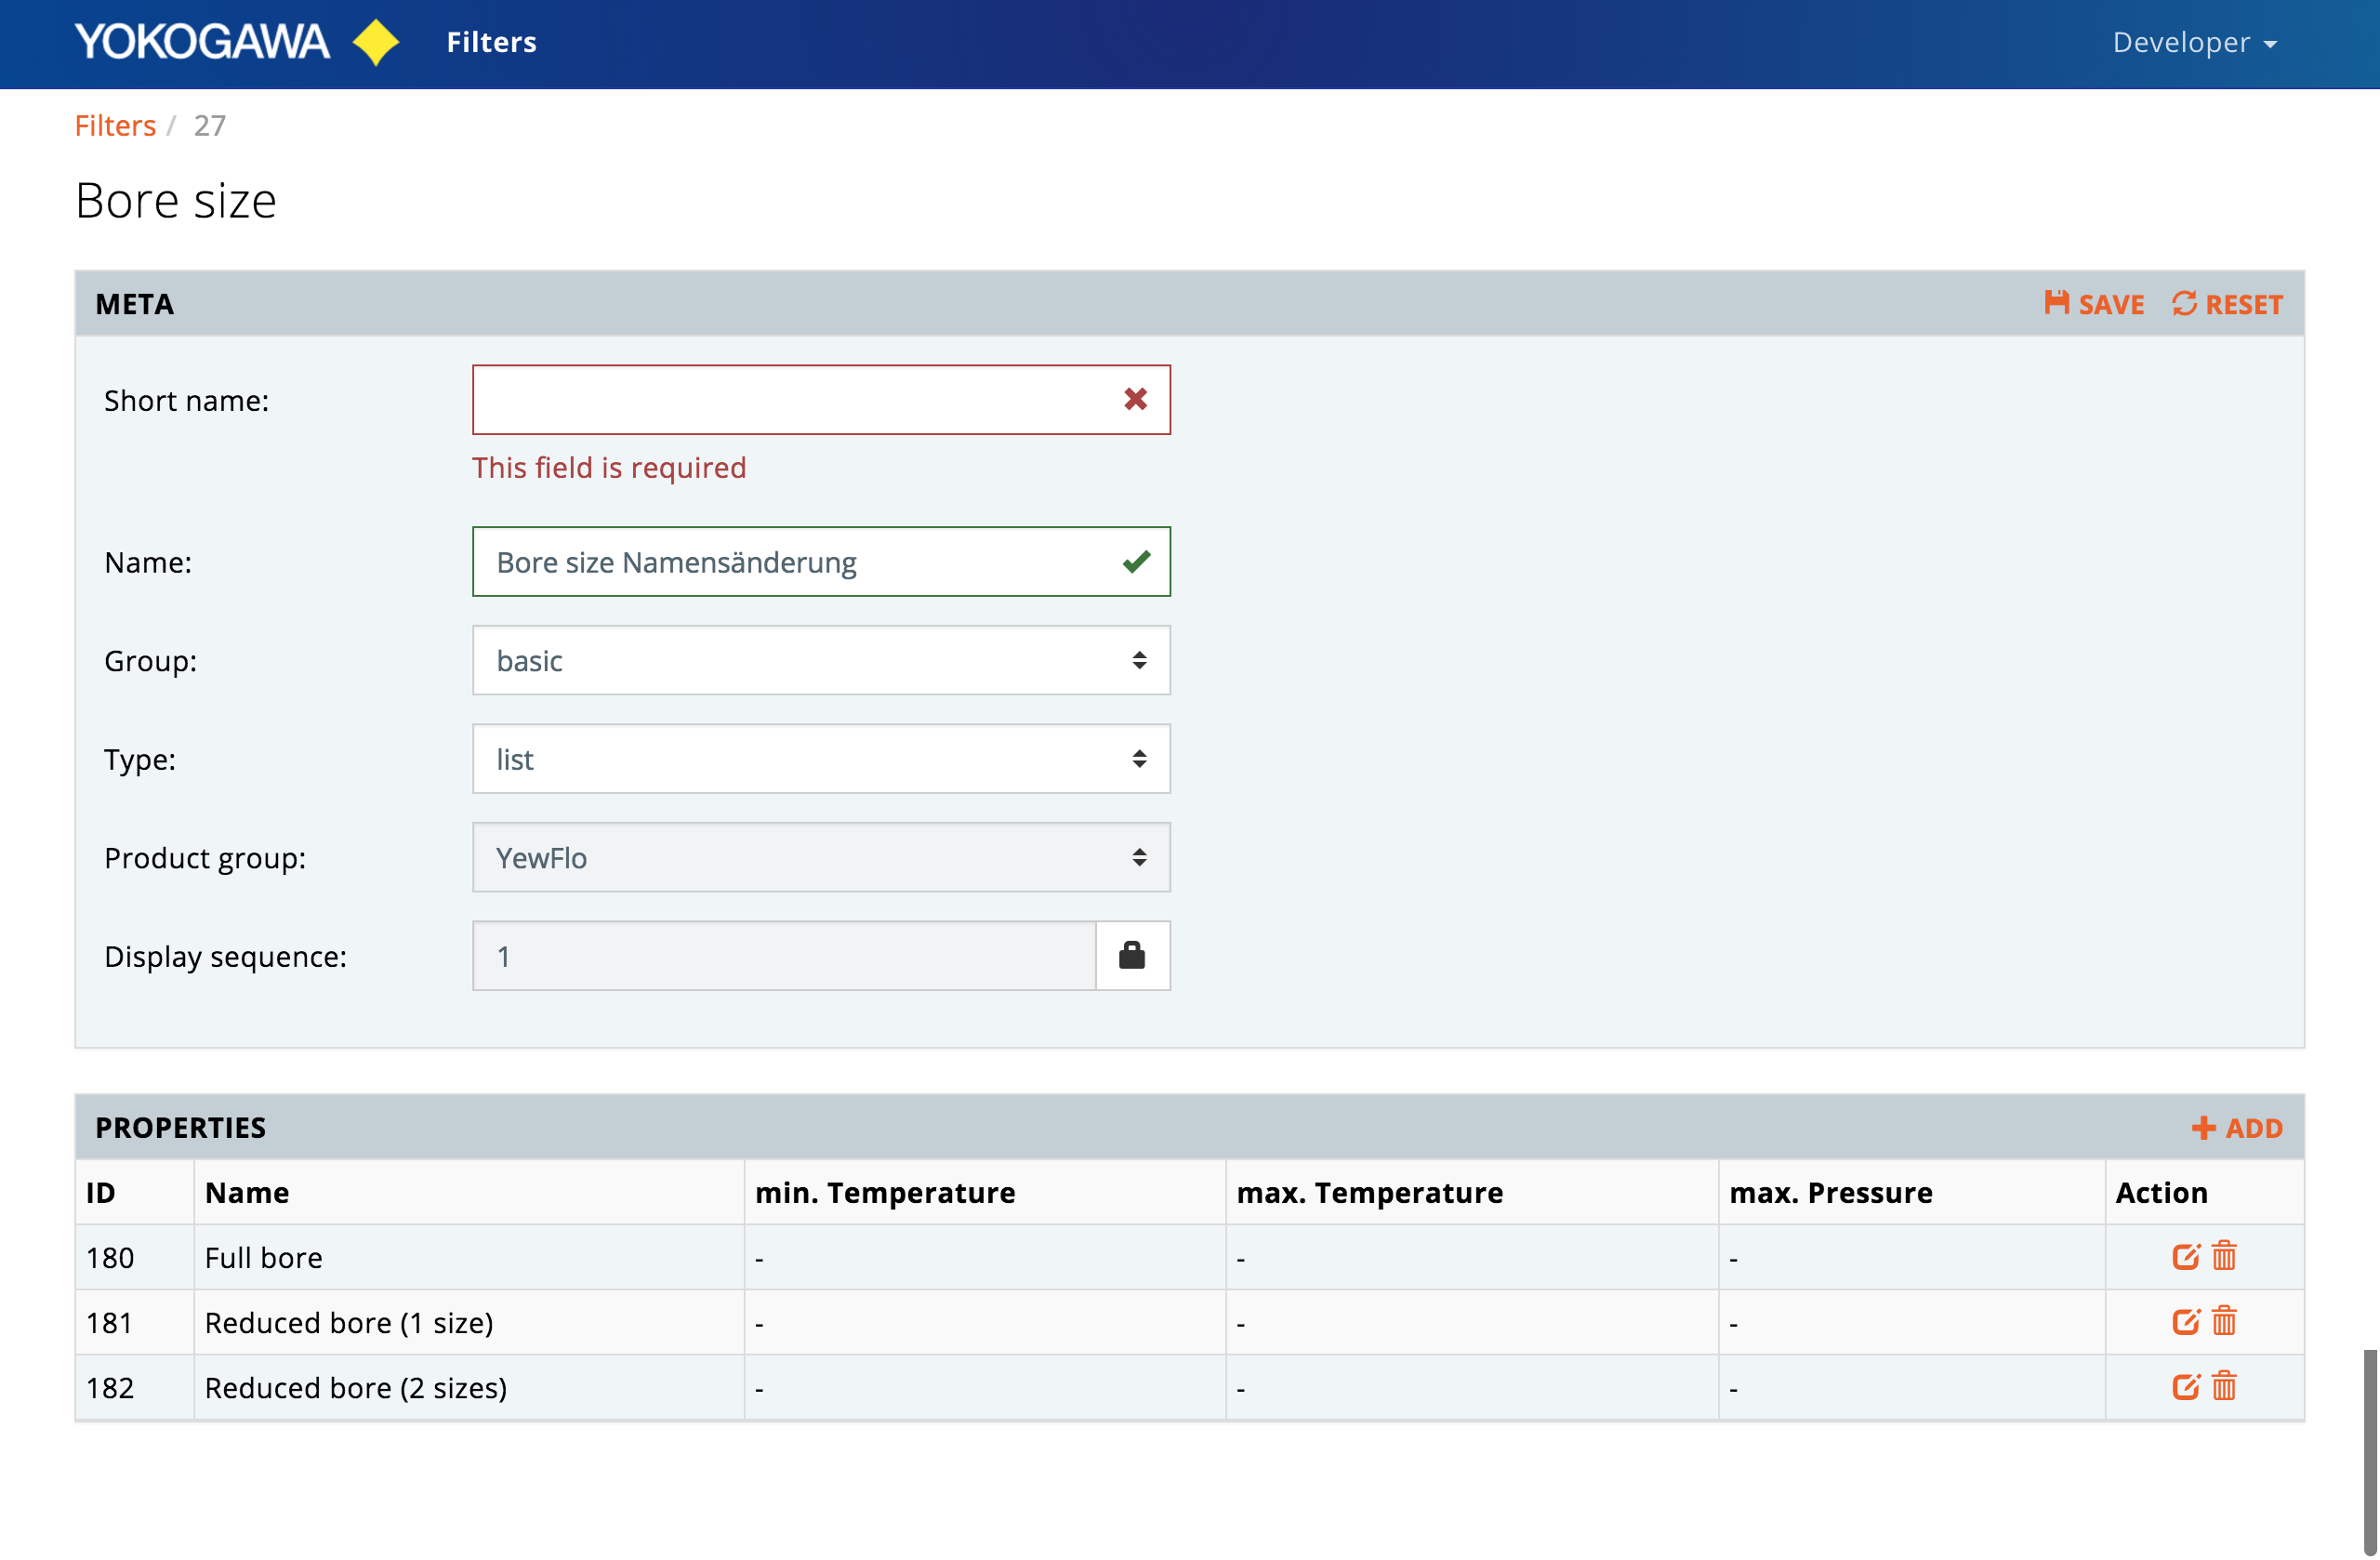
\includegraphics[width=1.0\textwidth]{ydm-edit} %{CS0031}
\caption{Screenshot einer Seite zum Bearbeiten von Filterdaten.}
\label{fig:editpage}
\end{figure}
Der Screenshot zeigt eine Seite zum Bearbeiten der Filterkerndaten. Diese Seite wird erreicht, indem der Benutzer auf den entsprechenden Bearbeiten-Button eines Filtersteuerelements klickt. Für die Gestaltung dieser Art von Seite, wurde sich an keiner konkreten Vorlage aus der FlowConfigurator Software orientiert. Es wurden aber dieselben übergreifenden Gestaltungsmerkmale und Stilmittel eingesetzt, die überall in der Webanwendung verwendet werden, um ein konsistentes Erscheinungsbild zu gewährleisten. Die dargestellte Seite zum Bearbeiten der Filterdaten realisiert Dateneingabemasken für die an einem Filterobjekt bearbeitbaren Daten. Außerdem wird über eine Tabelle die Abhängigkeit zu Properties hergestellt. Auf diesen lassen sich ebenfalls über nebenstehende Icons entsprechende Aktionen, auf Grundlage der gestellten funktionalen Anforderungen, ausführen. Als Beispiel wird in dem gezeigten Screenshot auch eine Validierung der eingegebenen Daten dargestellt, die in der gesamten Webanwendung in gleicher Art und Weise implementiert ist. Über die unter dem Header befindliche Breadcrumb-Navigation, erkennt der Benutzer, in welchem Schritt der Filterbearbeitung er sich gerade befindet. Entscheidet sich der Benutzer beispielsweise eine Property zu bearbeiten, erweitert sich diese Breadcrumb-Navigation und stellt zusätzlich die Möglichkeit bereit, zwischen einzelnen Bearbeitungsschritten zu navigieren. Die für die Erfüllung der restlichen funktionalen Anforderungen zu implementierenden Datenbearbeitungsseiten bauen alle auf ein ähnliches Layout auf und sind schrittweise über die bereitgestellten Kontextfunktionen erreichbar.
